\documentclass[a4paper,10pt]{article}
\usepackage[utf8x]{inputenc}
%\usepackage[french]{babel}
\usepackage{amsmath}
\usepackage{amsfonts}
\usepackage{amssymb}
\usepackage{graphicx}		 			% Inclusion des figures 
\usepackage{textcomp}
\usepackage[nointegrals]{wasysym}			% Collection de symboles mathématiques
\usepackage{multicol}					% Pour utiliser \hfill
\usepackage{ifthen}
\usepackage{tabularx}	 				% Gestion avancée des tableaux
%\usepackage[squaren]{SIunits}
%\usepackage{sistyle} 					% Mise en forme des unités
%\usepackage{fancyhdr} 					% Entêtes et pieds de pages personnalisés 
%\usepackage{latexsym}
%\usepackage{xcolor}					% Pour redéfinir des couleurs 
\usepackage[svgnames]{xcolor}				% Voir : http://calque.pagesperso-orange.fr/latex/latexps.html
\usepackage{latexsym}
\usepackage{fontenc}
\usepackage{wrapfig} 					% Pour pouvoir placer une image à côté de texte
\usepackage{cite}	
\usepackage{url} 					% Pour citer les sites internet dans la bilibographies
\usepackage{setspace}
\usepackage[T1]{fontenc}				% Indispendable, présent dans tous les codes exemples
\usepackage[linkcolor=red,colorlinks=true]{hyperref} 	% Hyper ref
\usepackage{listings}					% Pour citer du code
\usepackage[justification=centering]{caption}
\usepackage{subcaption}
\usepackage{subfloat}


\newcommand\pathpic{/home/nsaura/Documents/new_doc/Latex_files/Pic/BE_combustion/}
%\newcommand\spipath{/home/saura/Documents/Stage/Notes_Manip/Pic/Simu_pic/}

%%%%%%%%%% Raccourcis %%%%%%%%%%%
\newcommand{\lp}{\left(}
\newcommand{\rp}{\right)}
\newcommand{\rint}{\int^\infty_{-\infty}}
\newcommand{\dint}{\int^\infty_{0}}
\newcommand{\rsum}{\sum^\infty_{ j = -\infty}}
\newcommand{\cad}{c'est-à-dire}
\newcommand{\qcq}{quelconque}
\newcommand{\keps}{$k-\varepsilon$}
\newcommand{\chq}{$Ch_4$ }
\newcommand{\od}{$O_2$ }

%%% Couleurs %%%
\xdefinecolor{purple}{named}{MediumVioletRed}
\xdefinecolor{brick}{named}{DarkRed}
\xdefinecolor{forest}{named}{DarkMagenta}
\xdefinecolor{dgreen}{named}{DarkOliveGreen}
\xdefinecolor{darker}{named}{SaddleBrown}
\xdefinecolor{MidnightBlue}{named}{MidnightBlue}

\newcommand\brick{\color{brick}}
\newcommand\npurple{\color{forest}}
\newcommand\dgreen{\color{dgreen}}
\newcommand\darker{\color{Maroon}}
\newcommand\dblue{\color{MidnightBlue}}

\newcommand\black{\color{black}}
\newcommand{\bl}{\color{blue}}
\newcommand\red{\color{red}}

\usepackage{caption}
\usepackage[labelfont={color = Indigo, bf}, font = it ,justification=centering]{caption}
%%%%%%%%%%%%%%%%%%%

%opening
\title{ \dblue BE combustion : Flamme de diffusion turbulente }
\author{ \darker Patacini Lucas \& Saura Nathaniel}
\graphicspath{{\pathpic}, {/home/nsaura/Documents/new_doc/Latex_files/Pic/}}
\usepackage{geometry}
\geometry{hmargin=1.4cm, vmargin=1.2cm}

\begin{document}
\maketitle 
\vspace{-1cm}
\begin{figure}[ht!]
\centering
\includegraphics[height=3cm, width= 8cm]{\pathpic cover.png}
\end{figure}

\noindent La théorie de la combustion consiste en l’étude pour le contrôle des différents types de flammes dans des milieux de nature laminaire ou turbulente. \\
Pour obtenir une flamme il nous faut un comburant et un carburant. Dans notre cas, le dioxygène jouera le rôle de comburant et le méthane sera le carburant.
On distingue généralement deux types de flammes selon l’état de mélange des réactifs : si les réactifs sont pré-mélangés  avant d’être enflammés, on parlera de flamme de pré-mélange si par contre le mélange se fait dans le milieu ambiant et qu’il y a combustion on parlera de flamme de diffusion.\\

\noindent Dans ce BE, nous allons étudier une flamme de diffusion générée par l’injection de méthane dans l’air. Nous chercherons à étudier l’épaisseur ou la longueur de la flamme, également la température ou encore l’évolution de scalaire passif autour de la flamme. 

\section{Caractéristiques de la flamme}
\subsubsection*{Zone de combustion et flamme}
En suivant les indications de l’énoncé, nous obtenons une distribution de température typique de celle d’une flamme ; sur la figure (\ref{temp_flamme}), on distingue une zone nettement plus chaude que le reste du milieu qui est à température ambiante (300°K). La figure de droite de (\ref{carte_espece}) nous indique également que l'injection de méthane reste confinée au sein d'une forme conique. Dans cette zone d'injection, le méthane rencontre l'air ambiant augmentant de plus en plus les collisions entre les molécules augmentant la température. Lorsque cette température atteint une valeur critique c'est l'explosion thermique et les réactifs commencent à brûler. Il y a une concordance entre le déclin de la concentration de \chq (cf figure (\ref{carte_espece}) droite) et la zone de très forte température. Cette dernière correspond donc à la combustion du \chq et à l'apparition de la flamme. Comme nous l'avons fait remarquer lors de l'introduction, les réactifs sont mélangés dans le milieu de combustion, c'est donc une flamme de diffusion.	\\
Dans la fin de la zone rouge (figure ({\ref{temp_flamme})), la température décroît progressivement. Il n'y a plus de flamme ici car il n'y a plus de méthane à brûler (voir aussi figure (\ref{carte_espece})). La température se propage alors par diffusion moléculaire et par advection par la vitesse: les molécules proches du front de flamme (plus chaudes) transmettent une partie de leur énergie par collision avec des molécules plus loin du front donc plus froides et ce de proche en proche.

\begin{figure}[ht!]
\centering
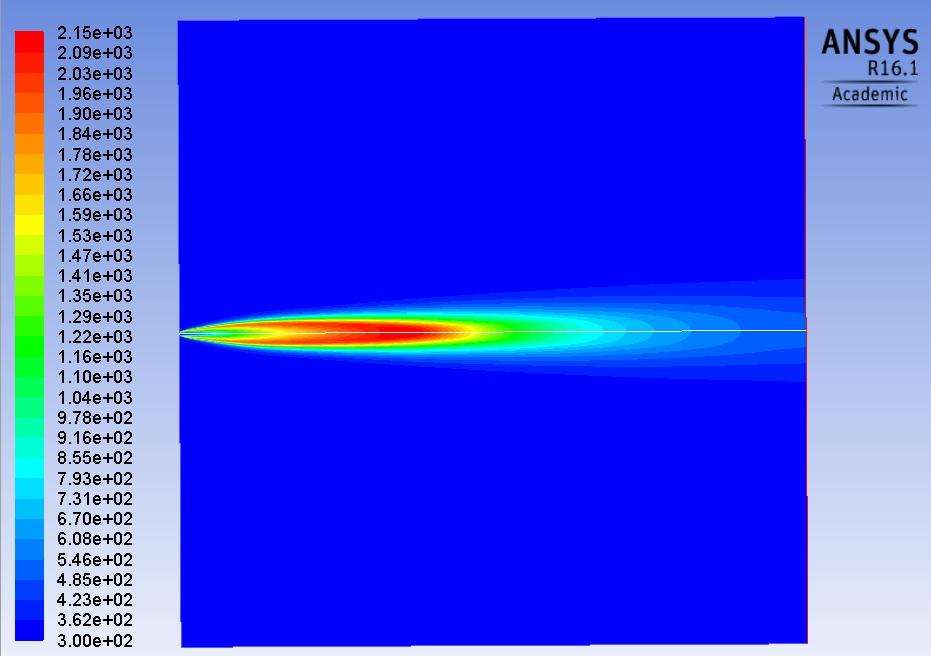
\includegraphics[scale= 0.35]{contour_temperature.jpg}
\caption{\footnotesize{Tracé du contour de la température symétrisé : on distingue clairement une zone plus chaude au centre, cette zone est la zone de combustion qui est caractérisé par une augmentation de la chaleur et la disparition de réactifs (transformés en produit). La température évolue de 300°K à environ 2160°K dans la zone la plus chaude de la flamme}}
\label{temp_flamme}
\end{figure}

\begin{figure}[ht!]

\includegraphics[height = 7cm, width=8.5cm]{\pathpic carte_o2.jpg} \hfill
\includegraphics[height = 7cm, width=8.5cm]{\pathpic carte_ch4.jpg}
\caption{Répartition des densités de l'\od (à gauche) et du \chq (à droite zoomé). La fraction massique de l'\od était initialement de 0.23 dans le milieu ambiant, la présence du jet de méthane implique donc une combustion de l'oxygène. Parallèlement, le méthane injecté "disparaît" peu à peu, il est aussi brûlé.}
\label{carte_espece}
\end{figure}
On peut lier les figures (\ref{temp_flamme}) et (\ref{carte_espece}). On remarque dans la figure (\ref{temp_flamme}) que la flamme commence vers les $x \approx 0.2$ zone ou les concentrations sont très basses. Comme nous avons vu dans le cours, la zone de réaction dans laquelle la température est la plus forte et dans laquelle on observe la flamme démarre lorsque les réactions entre les produits ont déjà bien commencé. Ces réactions augmentent petit à petit la température dans la zone où sont concentrés les réactifs, augmentant donc le nombre de molécules dépassant le seuil de l'énergie d'activation, augmentant ainsi le nombre de réactions. Puisqu'il y a plus de réactions, la température va encore augmenter et ainsi de suite. Ce processus de réactions en chaîne s'appelle l'explosion cinétique et explique que les concentrations des réactifs soient petites lorsque la flamme se déclenche. 

\darker \subsubsection*{Longueur et épaisseur de la flamme} \black
Pour évaluer la longueur de la flamme nous traçons la température sur l'axe des X=0 : 

\begin{figure}[ht!]
\centering
\includegraphics[scale=0.4]{\pathpic temperature_axe_X.jpg}
\caption{Évolution de la température le long de l'axe des X=0. La chute aux alentours de 0.4m reflète la position ou la flamme s'éteint. S'en suit une décroissance de la température selon une pente assez raide puis moins raide jusqu'à tendre vers 400°K environ.}
\label{temp_x0}
\end{figure}

\noindent Sur la figure (\ref{temp_x0}), on peut déterminer la longueur de la flamme. Elle est d'environ $L \approx 0.4 m$. Cette valeur est cohérente avec le cours ; en effet, pour une flamme de diffusion turbulente, on a .

\begin{equation}
L_{fl} \ \tilde{=} \ Cd_0
\label{loi_longueurflamme}
\end{equation}

\noindent Où $d_0$ est le diamètre de l'injecteur. Ici $d_0 = 4 mm$, on retrouve donc cette relation avec $$ L_{fl} = 100 d_0$$ Ce qui nous permet de valider nos résultat
\pagebreak

Pour déterminer l'épaisseur maximale de la flamme, on effectue des coupes verticales à des $x$ fixés et on trace l'évolution de la température en fonction de l'axe des $y$. les résultats de ces coupes sont disponibles figure (\ref{densite_temperature}).
\begin{figure}[ht!]
\centering
\includegraphics[scale=0.4]{\pathpic xy_densite_temp.png}
\caption{Tracé des température le long de l'axe $y$ (tronqué entre $0$ et $0.5$ car toutes les valeurs étaient zéro). On voit que pour $x=0.1$, la température est la plus élevée pour des $y$ légèrement décalées par rapport à l'axe des $X = 0$. Par contre en $x=0.4$, on peut dire que la flamme est sur l'axe des $X=0$.}
\label{densite_temperature}
\end{figure}

On voit que plus on s'approche des $x$ proche de la valeur de longueur de flamme, plus le pic de température se rapproche de l'axe $X=0$. Au-delà (courbe bleue sur la figure (\ref{densite_temperature}) la flamme étant éteinte, nous voyons l'air ambiant (et peut-être des produits brûlés) est chauffé par la conduction de chaleur des molécules proches de la flamme. À l'inverse, lorsque l'on effectue des coupes proche de l'origine du problème, les pics de température se situent plutôt plus loin de l'axe $Y=0$. On imagine donc une flamme conique d'épaisseur d'à peu près $0.05 \ m$ soit $5 \ cm$.

\darker \subsubsection*{Vitesse de flamme} \black
On va à présent estimer la vitesse de flamme. On trace dans un premier temps, la vitesse mesurée sur l'axe des $X=0$.

\begin{figure}[ht!]
\centering
\includegraphics[scale = 0.4]{\pathpic Vitesse_axe_X.png}
\caption{}
\label{}
\end{figure}

La première valeur est la vitesse d'injection du carburant à l'entrée. Par effet de viscosité de l'air et de son inertie, le carburant est freiné. Ce freinage augmente la température et les premières réactions commencent. Rapidement (aux alentours de $x \approx 0.1$), la vitesse change de comportement et commence à croître, jusqu'à arriver à un deuxième pic, moins grand que le premier, pour les $x \approx 0.4 \ m$. Puis elle décroît, sans s'annuler.\\
 On effectue des coupes le long de l'axe de $x$ pour différentes valeurs. Les tracés sont disponibles sur la figure (\ref{densite_vitesse}).
 
 \pagebreak
 \begin{figure}[ht!]
 \centering
 \includegraphics[scale=0.4]{\pathpic Vitesse_axe_Y.jpg}
 \caption{On distingue deux zones pour le tracé des vitesses : la première lorsque $y \leq 0.05$ correspond directement à l'injection d'air qui a provoqué la flamme. Dans la deuxième pour $y \geq 0.15$ on observerait plutôt les effets co-courant provoqué par la flamme générant de la vitesse pour l'air présent dans cette zone.} 
 \label{densite_vitesse}
 \end{figure}
 
 \noindent La figure précédente montre l'entraînement de l'air situé aux $y > 0.3$ (\cad $ $ loin de la flamme en elle même) par la flamme. On peut visualiser cette entraînement d'air en traçant les vecteurs vitesse dans toute la cuve, et en colorant leur magnitude par la concentration de $O_2$. On aura donc une meilleure vue de l'air entraîné par la flamme. Cet air entraîné alimente la flamme et pourrait même augmenter la longueur de la flamme, ou dans le cas contraire si la flamme est trop turbulente, créer des zones d'extinction.
 
  \begin{figure}[ht!]
 \centering
 \includegraphics[scale=0.4]{\pathpic vector_species_02.jpg}
 \caption{Meilleure visualisation de l'entraînement de l'air par la flamme. Au bout de paroi, on visualise un profil de vitesse similaire à un jet.}
 \label{vector_species}
 \end{figure}
 
 \darker \subsubsection*{Évolution du scalaire passif $z = Y_{ch_4} - \frac{Y_{0_2}}{4}$} \black
 Le scalaire passif est un bon moyen de connaître la richesse de mélange. Ici, on aurait besoin de 4 molécules de $0_2$ pour oxyder une molécule de $Ch_4$. D'après le cours, la flamme est délimité mour $Z = Z_{st}$ \cad $ $ lorsque le méthane est exactement oxydé par l'air. On trace alors le contour de ce scalaire avec des valeurs minimale et maximale pour observer l'action de la flamme.

 \pagebreak 

 \begin{figure}[ht!]
 \centering
 \includegraphics[scale=0.4]{\pathpic contour_scalaire_passif.PNG}
 \caption{}
 \label{}
 \end{figure}
 
\noindent On fait également des coupes pour différents x et on regarde l'évolution de scalaire en fonction de y.
 
  \begin{figure}[ht!]
 \centering
 \includegraphics[width = 11cm , height = 8cm]{\pathpic Capture_du_2017-02-03_12-52-22.png} \hfill
 \includegraphics[scale=0.2]{\pathpic cours.jpg}
 \caption{À gauche tracé du scalaire passif à différents $x$, à droite, section du cours illustrant le rapport entre la zone stœchiométrique et la longueur de flamme.}
 \label{scalaire_passif}
 \end{figure}

On voit alors que la flamme s'arrête légèrement avant $x=0.4$ car le scalaire passif n'est pas exactement égal à zéro. Cependant, la valeur de $z$ pour $x=0.4\ m$ est très petite de l'ordre de $10^{-3}$. Notre approximation sur la longueur de la flamme est donc valable.  \\
On peut également noter que dès lors que $y>0.05$, la valeur du scalaire est minimal, ce qui nous confirme notre valeur pour l'épaisseur de flamme.

\section*{Conclusion}
Dans ce BE nous avons pu étudier les différentes caractéristiques d'une flamme de diffusion. À partir d'une simulation numérique, nous avons pu exprimer la longueur, l'épaisseur et la vitesse de flamme. L'étude du scalaire passif $Z$ et notamment le contour $Z=0$, nous a permis de retrouver et donc de valider les valeurs de l'épaisseur et de la longueur de la flamme (voir figure (\ref{scalaire_passif})).\\
Nous avons mis en évidence l'action du jet de méthane sur l'air environnant : il est entraîné par convection libre dans la zone de combustion (voir figure (\ref{vector_species})). \\
Nous pourrions vérifier la loi donnée dans le cours (équation (\ref{loi_longueurflamme})) et valider et nuancer le coefficient obtenu lors de cette simulation.
\end{document}